\documentclass{beamer}
\usepackage[utf8]{inputenc}
\usetheme{Copenhagen}
%\usepackage[spanish]{babel}
\usepackage{multirow}
%\usepackage{estilo-apuntes}
%\usepackage{braids}
\usepackage[]{graphicx}
\usepackage{rotating}
\usepackage{pgf,tikz}
\usepackage{pgfplots}
\usepackage{tikz-cd}
\usepackage{mathtools}
%\usepackage{empheq}
%\usepackage[dvipsnames]{xcolor}
\usepackage{xcolor}
\usepackage{multicol}

\usetikzlibrary{arrows}
\usetikzlibrary{cd}
\usetikzlibrary{babel}
\pgfplotsset{compat=1.13}
%\usetikzlibrary{decorations.shapes}
%\pgfkeyssetvalue{/tikz/braid height}{1cm} %no parece hacer nada
%\pgfkeyssetvalue{/tikz/braid width}{1cm}
%\pgfkeyssetvalue{/tikz/braid start}{(0,0)}
%\pgfkeyssetvalue{/tikz/braid colour}{black}

\theoremstyle{definition}

\newtheorem{teorema}{Theorem}
\newtheorem{defi}{Definition}
\newtheorem{prop}[teorema]{Proposition}

\newcommand{\Z}{\mathbb{Z}}
\newcommand{\Q}{\mathbb{Q}}
\newcommand{\C}{\mathbb{C}}
\newcommand{\CC}{\mathcal{C}}
\newcommand{\D}{\mathbb{D}}
\providecommand{\gene}[1]{\langle{#1}\rangle}

\DeclareMathOperator{\im}{im}


\addtobeamertemplate{navigation symbols}{}{%
    \usebeamerfont{footline}%
    \usebeamercolor[fg]{footline}%
    \hspace{1em}%
    %\insertframenumber/\inserttotalframenumber
}
\setbeamercolor{footline}{fg=black}
\setbeamerfont{footline}{series=\bfseries}

\newcommand{\highlight}[1]{%
	\colorbox{red!50}{$\displaystyle#1$}}

\makeatletter
\newcommand*{\encircled}[1]{\relax\ifmmode\mathpalette\@encircled@math{#1}\else\@encircled{#1}\fi}
\newcommand*{\@encircled@math}[2]{\@encircled{$\m@th#1#2$}}
\newcommand*{\@encircled}[1]{%
	\tikz[baseline,anchor=base]{\node[draw,circle,outer sep=0pt,inner sep=.2ex] {#1};}}
\makeatother

\expandafter\def\expandafter\insertshorttitle\expandafter{%
  \insertshorttitle\hfill%
  \insertframenumber\,/\,\inserttotalframenumber}

%-----------------------------------------------------------

\title{Hastings Direct Exercise}
\author{Javier Aguilar Mart\'in}
\institute{University of Kent}
\date{}
 
\begin{document}
\frame{\titlepage}

\setbeamercovered{highly dynamic}

\newcounter{saveenumi}
\newcommand{\seti}{\setcounter{saveenumi}{\value{enumi}}}
\newcommand{\conti}{\setcounter{enumi}{\value{saveenumi}}}

\makeatletter
%\newcommand{\xRightarrow}[2][]{\ext@arrow 0359\Rightarrowfill@{#1}{#2}}
\makeatother

\resetcounteronoverlays{saveenumi}
%\AtBeginSection[]{
%\begin{frame}
%\frametitle{Tabla de contenidos}
%\tableofcontents
%\end{frame}
%}
\section{Dataset}

\begin{frame}
\frametitle{Task}
\begin{itemize}
\item<1-> Dataset of quotes for motor insurance returned by Hastings Direct.
\item<2-> Size: 50k rows and 19 columns. 
\item<3-> \textbf{Task}: explore, cleanse and analyze this dataset, and to then build a model to predict how much we should charge each customer.
\end{itemize}
\end{frame}



\begin{frame}
\frametitle{Columns}
\begin{minipage}{0.5\linewidth}
\begin{itemize}
 \item Quote\_ID
\item Quote\_Date
\item Driver1\_DOB
\item Driver1\_Licence\_Type
\item Driver1\_Licence\_Years
\item Driver2\_Licence\_Type
\item Driver2\_Licence\_Years
\item Driver1\_Convictions
\item Driver1\_Claims
\item Driver1\_Marital\_Status
\end{itemize}
\end{minipage}
\begin{minipage}{0.45\linewidth}
\begin{itemize}
\item Vehicle\_Age
\item Vehicle\_Value
\item Tax
\item Vehicle\_Annual\_Mileage
\item Credit\_Score
\item Payment\_Type
\item Days\_To\_Inception
\item Premium
\item Capped\_Premium
\end{itemize}
\end{minipage}
\end{frame}

\section{Cleansing and analysis}
\begin{frame}
\frametitle{Cleansing and analysis}
\begin{itemize}
\item<1-> Drop duplicates. Size reduced by a few hundreds.
\item<2-> $\text{Driver1\_Age} = \text{Quote\_Date} - \text{Driver1\_DOB}$ and
\item<2-> $\text{Driver1\_Age\_Start\_Licence} = \text{Driver1\_Licence\_Years} - \text{Driver1\_Age}$ (reduces correlation).
\item<3-> Drop Quote\_ID and Quote\_Date columns. %all dates are from 2020
\item<4-> Skip information about Driver2 for now.
\end{itemize}
\end{frame}


\begin{frame}
%how do they generalize associative algebras
\begin{itemize}
\item<1-> Replaces Driver1\_Convictions = \texttt{'-9999'} by \texttt{'No'}. %It's a yes or no column, innocent until proven guilty, data integrity
\item<2-> Reformat Driver1\_Marital\_Status for consistency. %some categories where capitalized other were not %tempting to drop but I keep it
\item<3-> Drop negative and extreme isolated values from Vehicle\_Age, Vehicle\_Value and Vehicle\_Annual\_Mileage %there were some jumps in the max value %very few, inputting with mean could be incorrect for extreme, but it's a possible option if concerned with data integrity
\item<4-> Drop Tax because it is a function of Vehicle\_Value %very high correlation confirms it
\end{itemize}
\end{frame}

\section{Distrbution}
\begin{frame}[fragile]
\frametitle{Some findings about the distribution} 

\begin{itemize}
\item<1-> Expect monthly payment to imply a higher premium than annual payments.
The box plot shows more than that.
\begin{center}
\item[]\includegraphics<2->[scale=0.3]{boxplot}
\end{center}
\end{itemize}
\end{frame}
\begin{frame}
\begin{itemize}
\item<1-> Assume Premium is the yearly payment. %the above investigation led me to this
\item<2-> Capped\_Premium is fixed and only applies when Premium $< 4000$, so drop it.
\item<3-> Days\_To\_Inception seems irrelevant as well, drop it. %always between 0 and 30 days, assume it is just time to start the insurance covering
\item<4-> Go back to drivers.
\end{itemize}
\end{frame}


\begin{frame}
\frametitle{Driver2}
\begin{itemize}
\item<1-> Assume no Driver2\_Licence\_Type and no Driver2\_Licence\_Years means no Driver2. 
\item<2-> This leads to a singles drivers model and a two drivers model.%more precision and data integrity, less data processing
\item<3-> The data for single drivers is clean, just drop Driver2 columns.
\end{itemize}
\end{frame}
\section{Feature extraction}
\begin{frame} 
\frametitle{Variation Inflation Factor}
%before modelling we need to extract the main features
\begin{itemize}
\item<1-> Premium will be the target value. The remaining columns are features.
\item<2-> Use VIF to eliminate most redundant numerical columns: 
\item[]<3-> Drop Vehicle\_Value %I would have expected others
\item<4-> 12 features in total, 10 for single drivers.
\end{itemize}
\end{frame}

\section{Modelling}
\subsection{Single drivers model}
\begin{frame}
\frametitle{Single drivers model}
\begin{itemize}
\item<1-> $>8k$ single drivers
\item<2-> Choose a tree based model: good for combination of categorical and numerical data.
\item<3-> Extrapolation problem can be dealt with by using a sufficiently large training set (80\%).
\item<4-> The data does not seem to follow clear patterns.
\begin{center}
\item[] \includegraphics<4->[scale=0.4]{scatter} %it is similar for all of them
\end{center}
\end{itemize}
\end{frame}


\begin{frame}
\frametitle{XGBoost Regressor}
\begin{itemize}
\item<1-> Choose XGBoost regressor: optimized tree based model.
\item<2-> Needed very little tuning.
\item<3-> $R^2=0.9999$, $MSE\approx 1$ vs $std\approx 1460$
\end{itemize}
\end{frame}

\begin{frame}
\frametitle{Actual vs predicted}
\begin{center}
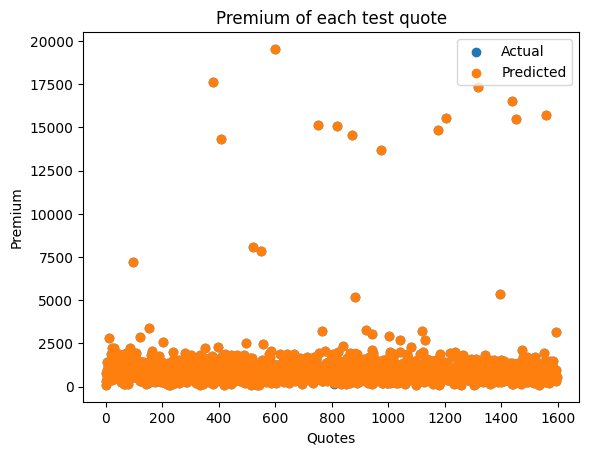
\includegraphics[scale=0.55]{singledrivers} %actual can't be seen
\end{center}
\end{frame}

\begin{frame}
\frametitle{Feature Importance}
\begin{center}
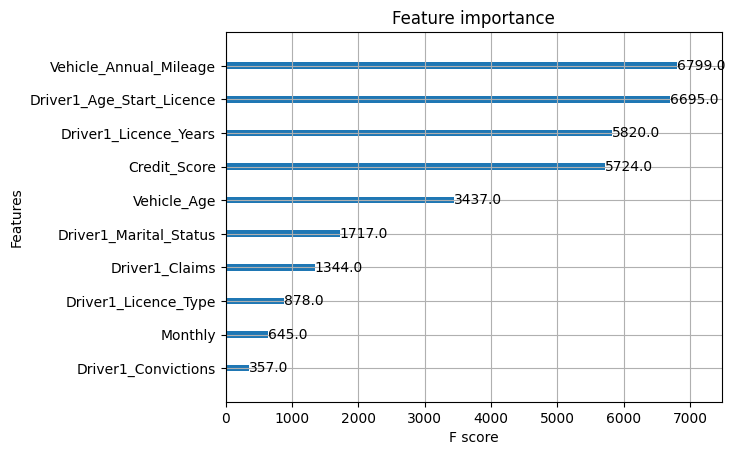
\includegraphics[scale=0.55]{singleimportance}
\end{center}
\end{frame}

\subsection{Two drivers model}
\begin{frame}
\frametitle{Two drivers model}
\begin{itemize}
\item $>40k$ pairs of drivers.
\item<1-> Consider missing Driver2\_Licence\_Type as its own category. %Like an 'Other' category
\item<2-> Fill Driver2\_Licence\_Years with average of its licence type or overall average otherwise. %would be useful to have other info
\item<3-> The model is now analogous to the single drivers. %alternatively both can be combined with another variable
\end{itemize}
\end{frame}

\begin{frame}
\frametitle{XGBoost performance}
\begin{itemize}
\item<1-> $R^2=0.9999$, $MSE<1$ vs $std\approx 11000$.
\item[]
\begin{center}
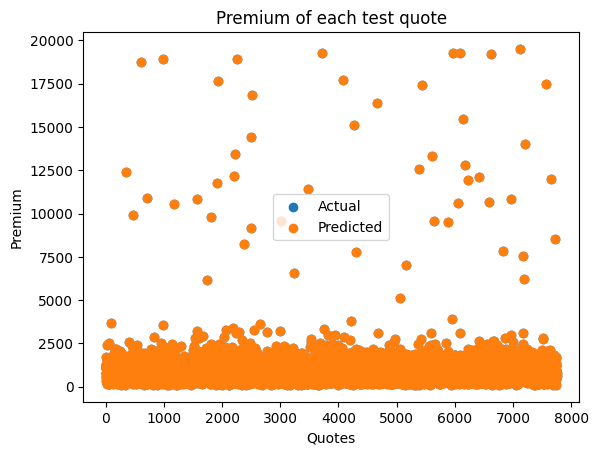
\includegraphics[scale=0.5]{twodrivers} %actual can't be seen
\end{center}
\end{itemize}
\end{frame}
\begin{frame}
\frametitle{Feature Importance}
\begin{center}
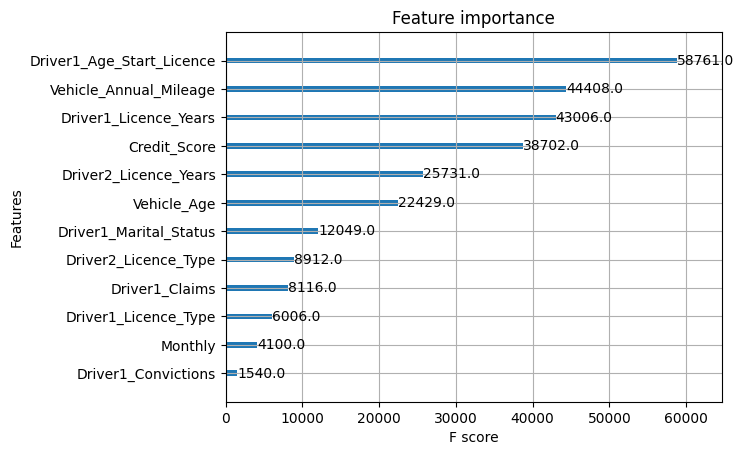
\includegraphics[scale=0.5]{twoimportance}
\end{center}
\end{frame}

\begin{frame}
\begin{center}
\Huge{Thank you!}
\end{center}
\end{frame}


\end{document}
